%----------------------------------------------------------------------------
\chapter{Evaluation}
%----------------------------------------------------------------------------
This chapter presents the applicability of the designed framework, evaluates its current capabilities and points out improvement possibilities.

%---------------------------------------------------------------
\section{The Oracle} \label{subs_evaloracle}
%---------------------------------------------------------------
%TODO: Optimistic vs Pessimistic, formalizmusok
The main metric of the oracle is the number of behavior-related questions the engineer has to answer during the course of the model synthesis (including the offline phase). This is really difficult to measure, as the exact number of these questions depends on several parameters: the complexity of the desired model, as well as the order, formalism, complexity and skillful construction of the requirements formulated by the designing engineer. Some of these parameters are difficult to measure by themselves, thus the following comparison of the supported formalisms is rather an illustration of the capabilities of the framework through a realistic example. 

For this demonstration, the traffic light component from the case study in Chapter \ref{sec_casestudy} is going to be used. We assume, that the user only adds requirements he perceives conducive to the model synthesis and tries to formulate realistic -- not unnecessarily complex -- requirements. 

The baseline of this experiment is the number of questions the user has to answer by always providing the corresponding outputs to the questions of the ILE, as higher numbers are the result of redundant requirements. We examine the cases when valid traces are also allowed, then add LTL expressions and finally invalid traces. Sequence diagrams are excluded from this comparison. The results can be seen on Figure \ref{fig_eval_trafficlightformalisms}.

\begin{figure}[H] 
	\centering
	%\fbox{
	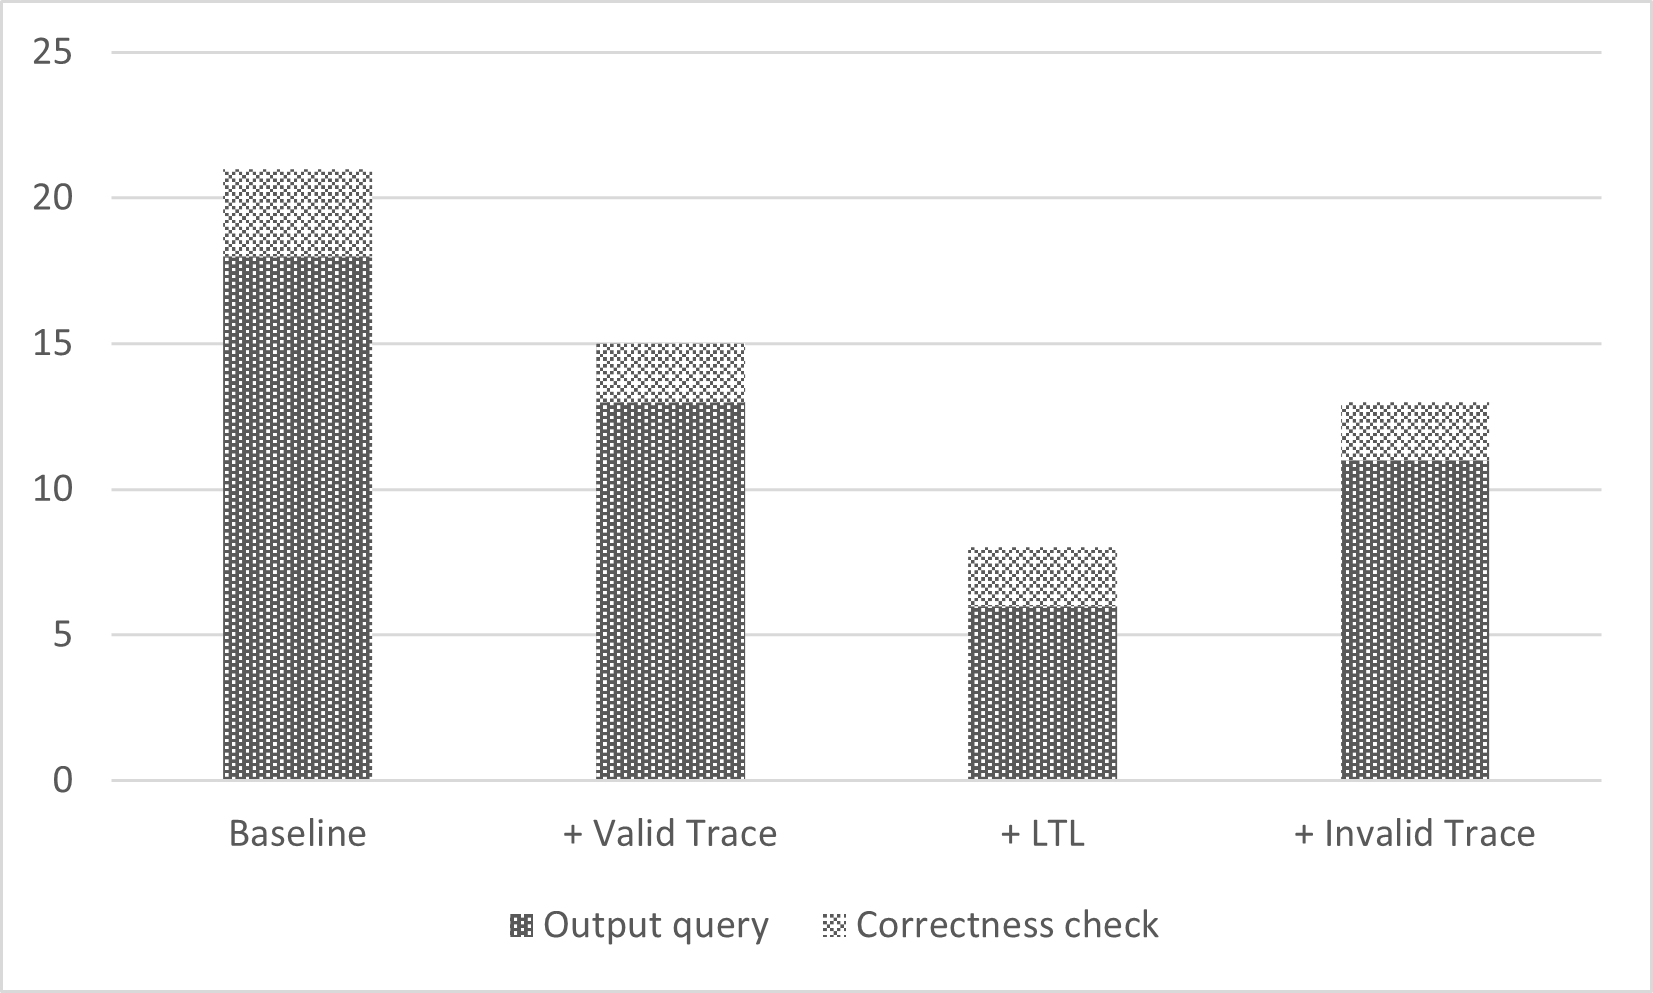
\includegraphics[width=130mm, keepaspectratio]{figures/evaluation_trafficlightformalism.png}
	%}
	\caption{Number of required interactions for modelling the traffic light component gradually extending the set of allowed formalisms} 
	\label{fig_eval_trafficlightformalisms}
\end{figure}

The requirements used in this experiment -- apart from the corresponding outputs answering the questions of the ILE directly -- can be seen in [TODO appendix]. The smallest number of queries was measured when both valid traces and LTL expressions were used. The addition of invalid traces resulted in a slightly higher number, demonstrating that this formalism is difficult to apply and useful mostly for its other benefits.  
 
%---------------------------------------------------------------
\section{The Learning Algorithm} \label{subs_evallearningalgo}
%---------------------------------------------------------------
%TODO: Optimistic vs Pessimistic, minimization
The runtime of the \textit{Adaptive Learning Algorithm} depends on the adaption commands provided. 

The Direct Hypothesis Construction algorithm, which, as theorized and proved in \cite{Steffen2011} and \cite{10.1007/978-3-642-34781-8_19}, terminates after at most $n^3mk+n^2k^2$ membership, and $n$ equivalence queries, where $n$ is the number of states of the canonical acceptor of the system under learning, $k$ is the size of the input alphabet and $m$ is the longest counterexample. The utilized suffix handling proposed by Rivest and Schapir\cite{rivest1993inference}, adds only one suffix to the set of suffixes in each learning round, so $m=1$\cite{Steffen2011}. As opposed to the traditional DHC, the Adaptive DHC can have more than $n$ learning rounds (but not more than $n$ equivalence queries) as a result of the $RESET$ command. Let $r$ be the total number of reset commands the algorithm receives. As seen in \cite{Steffen2011}, the set of suffixes is bound by $k+mn$, or in this case, $k+1*(n+r)$. Since the number of transitions needed to consider never exceed $nk$\cite{Steffen2011}, and the maximum number of equivalence queries is $n$, the maximum number of membership queries of the \textit{Adaptive Learning Algorithm} is $(k+n+r)*nk*n = $\textbf{$ n^2k^2+n^3k+n^2kr$}.

When \textit{PESSIMISTIC} commands are used, the number of equivalence queries get closer to $n$, but the number of \textit{new} membership queries only increase by $k$. Conversely, \textit{OPTIMISTIC} commands reduce the number of equivalence queries needed, but increase the membership queries in the learning round.
%---------------------------------------------------------------
\section{Caching} \label{subs_evalcaching}
%---------------------------------------------------------------
%TODO: optimisticre mennyit csökkent, RESET

The implemented memoization, which utilizes a radix tree, has many advantages in both run- and space complexity. TODO